\documentclass[9pt,a4paper,twocolumn,twoside]{rho-class/rho}
\usepackage[english]{babel}

% Figures are generated once by the pipeline into reports/figures/ and read
% directly from there - no duplicate copy is kept under reports/doc/.
\graphicspath{{../figures/}}

%----------------------------------------------------------
% Title
%----------------------------------------------------------

\doctype{Machine Learning Capstone - Technical Report}
\title{Jet Engine Hospital: A Leakage-Safe Multi-Task Early-Warning System for NASA C-MAPSS Turbofan Engines}

%----------------------------------------------------------
% Authors, Affiliations and dates
%----------------------------------------------------------

\author[{\textasteriskcentered},a,1]{Ehsan R Habibagahi}

%----------------------------------------------------------

\affil[a]{Department of Computer Science, Shahid Beheshti University}

%----------------------------------------------------------

\dates{This manuscript reports on work completed for the Machine Learning capstone, Spring 2026}

%----------------------------------------------------------
% Corresponding author-, Document- information
%----------------------------------------------------------

\corres{\textsuperscript{\textasteriskcentered}Corresponding author: \href{mailto:habibagahiehsan25@gmail.com}{habibagahiehsan25@gmail.com}.}

%----------------------------------------------------------

\docinfo{Instructor: Dr. Farahani. All notebook, application and evaluation code referenced in this report is included in the accompanying submission and runs top-to-bottom from the raw NASA C-MAPSS release.}

%----------------------------------------------------------

\journalname{Shahid Beheshti University}
\journal{Machine Learning Capstone, Spring 2026}
\theday{\today}
\vol{1}
\no{1}

%----------------------------------------------------------
% Abstract and Keywords
%----------------------------------------------------------

\begin{abstract}
    We present Jet Engine Hospital, a multi-task early-warning system for the NASA C-MAPSS turbofan degradation benchmark. The system estimates remaining useful life (RUL) with a calibrated, adaptive-width prediction interval; predicts failure within 10, 20 and 30-cycle horizons with calibrated probabilities; detects abnormal behaviour with four unsupervised detectors trained without failure labels; and converts all three signals into an auditable CONTINUE / INSPECT / STOP maintenance recommendation under an explicit asymmetric cost. The entire pipeline enforces an engine-level train/validation/test split before any preprocessing is fitted, and every causal feature is verified - not merely assumed - to depend only on present and past cycles. On the Stage 1 foundation subset (FD001) the deployed model reaches a test MAE of 8.21 cycles and a 90\% adaptive prediction interval with 93.3\% empirical coverage; the 20-cycle failure classifier reaches PR-AUC 0.884; the best anomaly detector separates near-failure from healthy engines with a validation-tuned alert rule that achieves zero missed warnings among at-risk test engines. Stressing the identical protocol on FD002 (six operating conditions) and FD003 (two fault modes) shows that condition shift and multi-fault degradation are separable failure modes for the method, while the FD004 bonus subset - which combines both stressors - degrades classification performance (PR-AUC at 20 cycles falls to 0.739) by substantially more than the sum of the two individual effects, evidencing a genuine interaction rather than additive difficulty.
\end{abstract}

%----------------------------------------------------------

\keywords{Predictive Maintenance, Remaining Useful Life, NASA C-MAPSS, Conformalized Quantile Regression, Anomaly Detection, Prognostics and Health Management}

%----------------------------------------------------------

\begin{document}

    \maketitle
    \thispagestyle{firststyle}

%----------------------------------------------------------

\section{Problem Framing}

    \rhostart{J}et engines degrade gradually and unobservably until a fault becomes measurable in the sensor stream, after which failure follows within a bounded number of operating cycles. NASA's Commercial Modular Aero-Propulsion System Simulation (C-MAPSS) benchmark \cite{saxena2008damage,saxena2008cmapss,frederick2007cmapss} simulates exactly this process: each engine is a separate multivariate time series recording three operating settings and 21 sensor channels per cycle, beginning at an unknown level of initial wear and ending at failure. Training trajectories run to failure; test trajectories are truncated at an arbitrary point before failure, with the true remaining cycle count supplied separately.

    The objective of this project is not to minimise one headline metric but to build a maintenance decision system whose data split, feature causality, uncertainty and cost trade-offs survive technical review. Three complementary model families are required: a regression model estimating $\mathrm{RUL}(i,t) = T(i) - t$ with a calibrated interval; three classifiers predicting $\Pr(\mathrm{RUL}(i,t) \le h)$ for $h \in \{10,20,30\}$; and an unsupervised anomaly score fitted without ever consulting a failure label. All three are combined into one auditable recommendation whose thresholds are learned exclusively on held-out validation engines and whose triggering rule is always reported alongside the recommendation.

    \begin{rhoenv}[frametitle=Two-stage design]
        Stage 1 (foundation) uses FD001 - one operating condition, one fault mode. Stage 2 stresses the identical protocol on FD003 (the graded subset: one condition, two fault modes) with FD002 (six conditions, one fault mode) run as a companion to separate the condition-shift stressor from the multi-fault stressor. FD004 (six conditions, two fault modes) is the bonus subset, combining both stressors under the same locked protocol.
    \end{rhoenv}

    The full pipeline - data loading through final comparison - lives in one importable Python package (\texttt{jeh}), built on scikit-learn \cite{pedregosa2011scikit}, and is imported identically by the analysis notebook and the deployed dashboard, so that the two are provably consistent rather than merely similar (Section~\ref{sec:app}). Every reported number in this report is reproduced from that package with a fixed random seed.

\section{Dataset and Data Audit}

    \tabref{tab:subsets} summarises the four official subsets used in this study. FD002 and FD004 contain six operating regimes (sea level through cruise), which is the axis of difficulty absent from FD001 and FD003; FD003 and FD004 contain two independent fault mechanisms (HPC and fan degradation), which is the axis absent from FD001 and FD002.

    \begin{table}[H]
        \caption{Official C-MAPSS subsets and their role in this study.}
        \label{tab:subsets}
        \begin{tabular}{
            >{\raggedright\arraybackslash}p{0.10\columnwidth}
            >{\raggedright\arraybackslash}p{0.15\columnwidth}
            >{\raggedright\arraybackslash}p{0.13\columnwidth}
            >{\raggedright\arraybackslash}p{0.42\columnwidth}
        }
        \toprule
        \textbf{Subset} & \textbf{Engines (tr/te)} & \textbf{Cond. / Fault} & \textbf{Role} \\
        \midrule
        FD001 & 100 / 100 & 1 / 1 & Stage 1 foundation \\
        FD002 & 260 / 259 & 6 / 1 & Stage 2, condition shift \\
        FD003 & 100 / 100 & 1 / 2 & Stage 2, multi-fault (graded) \\
        FD004 & 248 / 249 & 6 / 2 & Bonus, combined challenge \\
        \bottomrule
        \end{tabular}
        \tabletext{Note: ``Cond.\ / Fault'' gives the number of operating conditions and fault modes.}
    \end{table}

    Row- and engine-level auditing (performed separately for the official train and test files, and again after the engine-level split) found zero missing values, zero non-finite values, zero duplicate $(\text{engine\_id}, \text{cycle})$ keys, and gap-free cycle indices starting at 1 for every engine in every subset. FD001 engine lifetimes range from 128 to 362 cycles (median 199), nearly a $3\times$ spread driven entirely by unknown initial wear, which is the direct argument against using raw cycle count as a predictive feature.

    A per-subset variance check on \emph{training} engines only removes near-constant sensor channels before any downstream fitting: seven sensors are dropped on FD001 (\texttt{sensor\_1,5,6,10,16,18,19}), five on FD003, and only two (\texttt{sensor\_16,19}) on FD002/FD004 - channels that are dead under one operating condition often carry regime information under six. Re-deriving this list per subset, rather than reusing FD001's, is necessary for correctness on the condition-rich subsets. \figref{fig:trajectories} shows representative raw sensor trajectories: several sensors trend upward toward failure while others trend downward, confirming that the model cannot assume a single degradation direction and must consume signed, regime-normalised residuals.

    \begin{figure}[H]
        \centering
        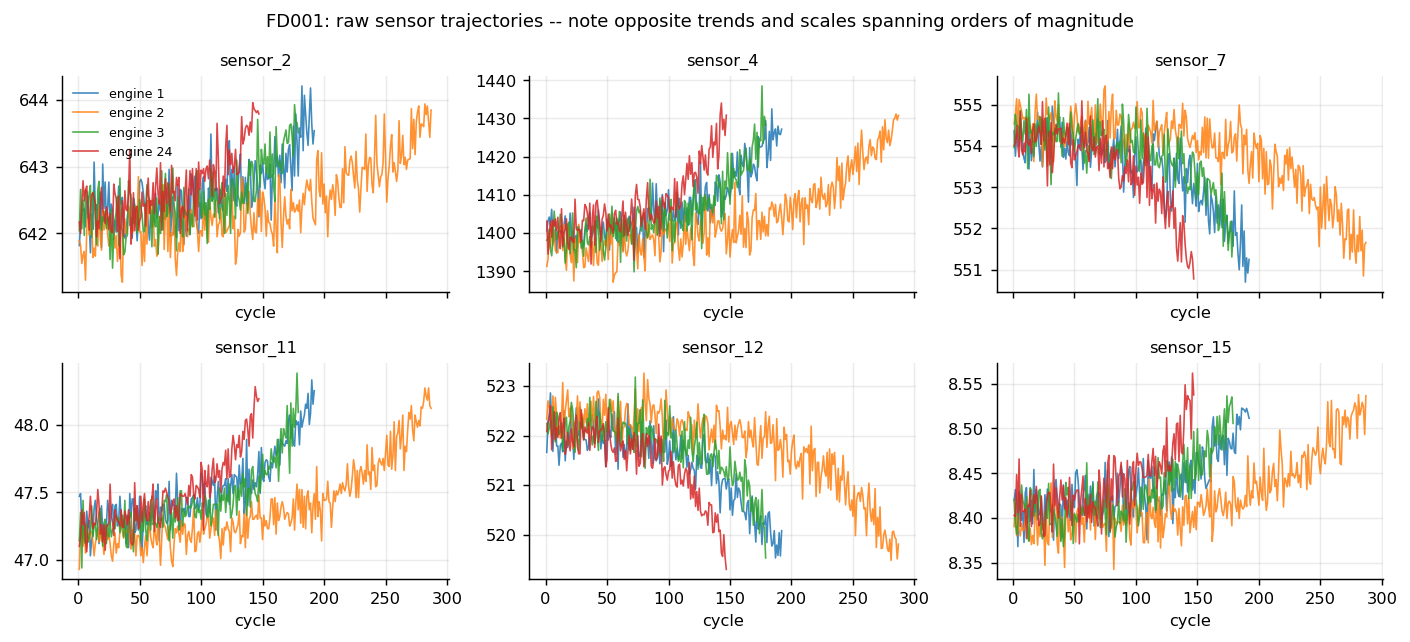
\includegraphics[width=\columnwidth]{FD001_trajectories.png}
        \caption{Raw sensor trajectories for four FD001 training engines. Degradation direction and scale differ substantially across channels, motivating regime-normalised, signed feature construction.}
        \label{fig:trajectories}
    \end{figure}

    Class balance after the engine-level split is severe and horizon-dependent: on FD001 test rows, the 10-cycle positive rate is 0.13\% (17 of 13{,}096 rows, an imbalance ratio of 769:1), rising to 0.94\% at 20 cycles and 2.54\% at 30 cycles. This motivates PR-AUC over ROC-AUC or accuracy throughout Section~\ref{sec:classification}.

\section{Leakage-Safe Evaluation Protocol}
\label{sec:protocol}

    The core constraint governing every experiment is that the engine-ID split is fixed \emph{before} any preprocessing, feature selection, window construction or threshold tuning occurs. \tabref{tab:protocol} states the allowed data at each stage.

    \begin{table}[H]
        \caption{The locked evaluation protocol.}
        \label{tab:protocol}
        \begin{tabular}{
            >{\raggedright\arraybackslash}p{0.20\columnwidth}
            >{\raggedright\arraybackslash}p{0.15\columnwidth}
            >{\raggedright\arraybackslash}p{0.35\columnwidth}
        }
        \toprule
        \textbf{Step} & \textbf{Data} & \textbf{Enforcement} \\
        \midrule
        Split IDs & engine\_id only & disjoint sets, saved to disk \\
        Fit preprocessing & train engines & scaler, regime clusters, sensor drop list \\
        Build windows & within split & per-engine grouping only \\
        Tune / calibrate & validation & RUL cap, thresholds, intervals \\
        Final evaluation & test engines & one locked pipeline, evaluated once \\
        \bottomrule
        \end{tabular}
    \end{table}

    Test engines are the official, failure-truncated \texttt{test\_FDXXX.txt} trajectories with RUL supplied by \texttt{RUL\_FDXXX.txt}; they are touched exactly once for final reporting. The official training engines are further split 70/30 by engine ID into a training set (used to fit the feature pipeline and every model) and a validation set (used for RUL-cap estimation, decision thresholds, isotonic calibration, and conformal quantiles). \tabref{tab:splitsizes} gives the resulting sizes.

    \begin{table}[H]
        \caption{Engine-level split sizes by subset.}
        \label{tab:splitsizes}
        \begin{tabular}{lrrr}
        \toprule
        \textbf{Subset} & \textbf{Train} & \textbf{Val.} & \textbf{Test} \\
        \midrule
        FD001 & 70 & 30 & 100 \\
        FD002 & 182 & 78 & 259 \\
        FD003 & 70 & 30 & 100 \\
        FD004 & 174 & 75 & 248 \\
        \bottomrule
        \end{tabular}
    \end{table}

    \begin{rhoenv}[frametitle=Causality test]
        For any feature at cycle $t$, changing rows after $t$ must not change that feature's value. This is not assumed: for a probe engine and cycle in every subset, the pipeline recomputes features from the full history and from a history truncated at $t$, and asserts the two are bit-identical. The one non-obvious case is the ``drift from baseline'' feature, whose baseline is an \emph{expanding} mean that freezes after 5 cycles rather than a plain first-5-cycles mean - a row at cycle 2 must not see cycle 5.
    \end{rhoenv}

\section{Time-Series Feature Engineering}

    Every sensor's regime-normalised residual is expanded into a current-cycle value plus a trailing-window representation at three window lengths (5, 15, 30 cycles): rolling mean and standard deviation at each length, rolling min/max, an OLS trend slope computed from rolling moments, an exponentially-weighted mean, a first difference, and a drift term relative to the engine's own frozen early-life baseline (cancelling unknown initial wear). All statistics are strictly trailing (\texttt{rolling(..., center=False)}); none use the engine's final cycle. For FD002/FD004, sensor residuals are computed \emph{within} a k-means-discovered operating regime (fit on the three operating settings, standardised, on training engines only) rather than globally, because the between-regime sensor variance otherwise dwarfs the within-regime degradation signal.

    The resulting feature space has 201 columns on FD001, 229 on FD003, and 277 on FD002/FD004 (the larger subsets add per-regime one-hot context and retain more sensors, since fewer channels are near-constant under six conditions).

\section{RUL Regression}
\label{sec:rul}

    \subsection{Piecewise Cap: Estimated, Not Grid-Searched}

        A piecewise-linear RUL target - constant while an engine is healthy, linear once degradation is observable - is standard practice, but the cap value cannot be chosen by grid-searching validation error: clipping predictions at a low cap structurally bounds the achievable error and mechanically favours the smallest candidate, particularly under the PHM asymmetric score (Section~\ref{sec:asymcost}), which specifically penalises RUL over-estimation. An early implementation that grid-searched the cap selected 60 cycles and reported a spuriously small MAE dominated by rows sitting on a constant target.

        The cap is instead \emph{estimated} from a degradation-onset analysis on training engines, without consulting any RUL label: the first principal component of the regime-normalised sensor residuals (oriented to increase with cycle index) is smoothed and compared against each engine's own first-30-cycle baseline; onset is the first cycle where the index exceeds baseline mean $+\,3\sigma$ persistently (3 of the last 5 cycles). The deployed cap is the median RUL-at-onset across training engines, snapped to a reporting grid. This produces caps of 130 (FD001), 110 (FD002), 125 (FD003) and 125 (FD004) - independently converging on the value ($\approx$125) widely assumed in published C-MAPSS work, while remaining derivable per subset.

    \subsection{Model Comparison}

        Six regressors are compared under identical splits and features: Ridge and polynomial Ridge on current-cycle-only features, Ridge/Random Forest \cite{breiman2001random}/Gradient Boosting \cite{friedman2001greedy}/Hist Gradient Boosting on the full window representation. \tabref{tab:reg_fd001} reports FD001 test-set performance; the deployed model on every subset is selected by validation MAE, not the PHM score, because the PHM score's exponential penalty rewards models that are uniformly pessimistic about RUL rather than accurate - on FD004 this selected the weakest model in the zoo (\texttt{ridge\_current}) during development, which was corrected before final results were produced.

        \begin{table}[H]
            \caption{RUL regression, FD001 test engines (all rows).}
            \label{tab:reg_fd001}
            \begin{tabular}{lrrrr}
            \toprule
            \textbf{Model} & \textbf{View} & \textbf{MAE} & \textbf{RMSE} & \textbf{R\textsuperscript{2}} \\
            \midrule
            HistGB     & window  & \textbf{8.21} & \textbf{12.21} & \textbf{0.827} \\
            GradBoost  & window  & 8.29 & 12.11 & 0.830 \\
            RandForest & window  & 9.49 & 13.06 & 0.802 \\
            RandForest & current & 10.88 & 16.70 & 0.677 \\
            Ridge      & window  & 11.23 & 15.38 & 0.726 \\
            Ridge(deg2)& current & 12.82 & 18.08 & 0.621 \\
            Ridge      & current & 13.85 & 19.24 & 0.571 \\
            \bottomrule
            \end{tabular}
            \tabletext{Note: HistGB is selected on validation MAE and deployed; ``view'' contrasts current-cycle-only features against the full trailing-window representation.}
        \end{table}

        Swapping only the feature view (Ridge current $\to$ Ridge window; Random Forest current $\to$ window) cuts MAE substantially with the model class held fixed, confirming that degradation lives in the trend rather than the instantaneous reading. The gap between linear and tree-based models on the same window features is real but smaller than the feature-view gap.

    \subsection{Where the Error Lives}

        \tabref{tab:region} breaks FD001 test error down by life region. Near-failure error is lowest and least late-biased - the desirable ordering for a maintenance-relevant metric, since a model that is accurate everywhere except near failure would be dangerous regardless of its headline MAE. Early-life R\textsuperscript{2} is negative because the target is a near-constant cap there, so low error in that region reflects target simplicity, not model skill.

        \begin{table}[H]
            \caption{FD001 test error by life region.}
            \label{tab:region}
            \begin{tabular}{lrrrr}
            \toprule
            \textbf{Region} & \textbf{Rows} & \textbf{MAE} & \textbf{Late frac.} & \textbf{R\textsuperscript{2}} \\
            \midrule
            Early-life (RUL$\ge$80)   & 11{,}061 & 1.44 & 0.022 & $-5.70$ \\
            Mid-life (30-80)         & 1{,}728  & 8.34 & 0.753 & 0.468 \\
            Near-failure ($<$30)      & 307      & 3.62 & 0.616 & 0.367 \\
            \bottomrule
            \end{tabular}
        \end{table}
        
        \figref{fig:residuals} shows the corresponding residual diagnostics: the model is mildly conservative overall (mean residual $-1.48$ cycles on FD001), the safe direction under the cost policy in Section~\ref{sec:asymcost}.

        \begin{figure}[H]
            \centering
            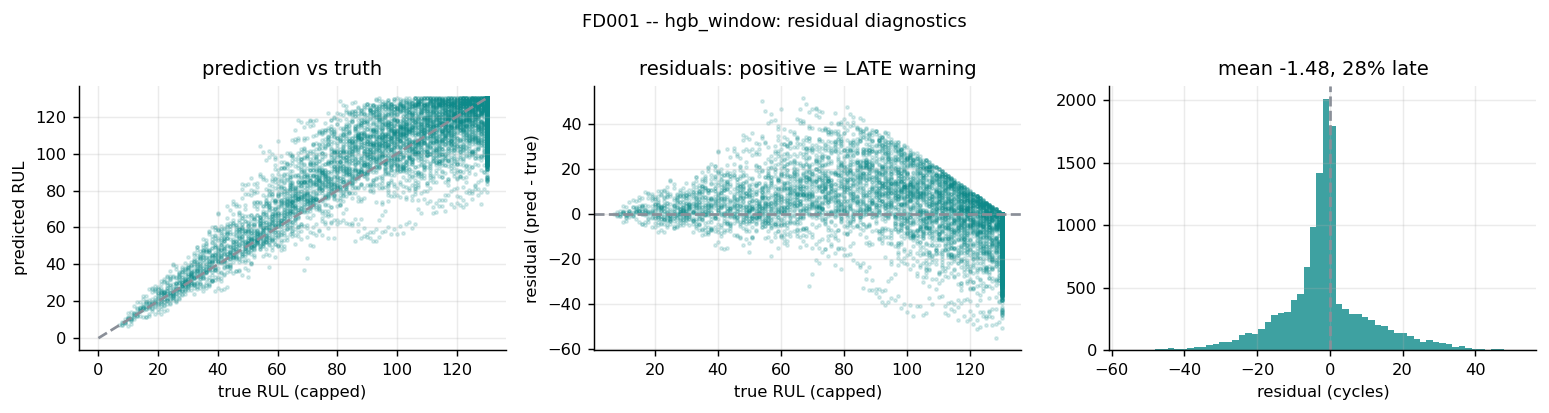
\includegraphics[width=\columnwidth]{FD001_residuals.png}
            \caption{FD001 residual diagnostics for the deployed regressor. Positive residuals (over-estimated RUL) correspond to late warnings.}
            \label{fig:residuals}
        \end{figure}

        A fleet average can hide catastrophic engines: the per-engine MAE distribution (\figref{fig:perengine}) is right-skewed, and the worst FD001 test engine's MAE is several times the fleet mean - which is why the decision policy in Section~\ref{sec:policy} keys off the calibrated \emph{lower} bound rather than the point estimate.

        \begin{figure}[H]
            \centering
            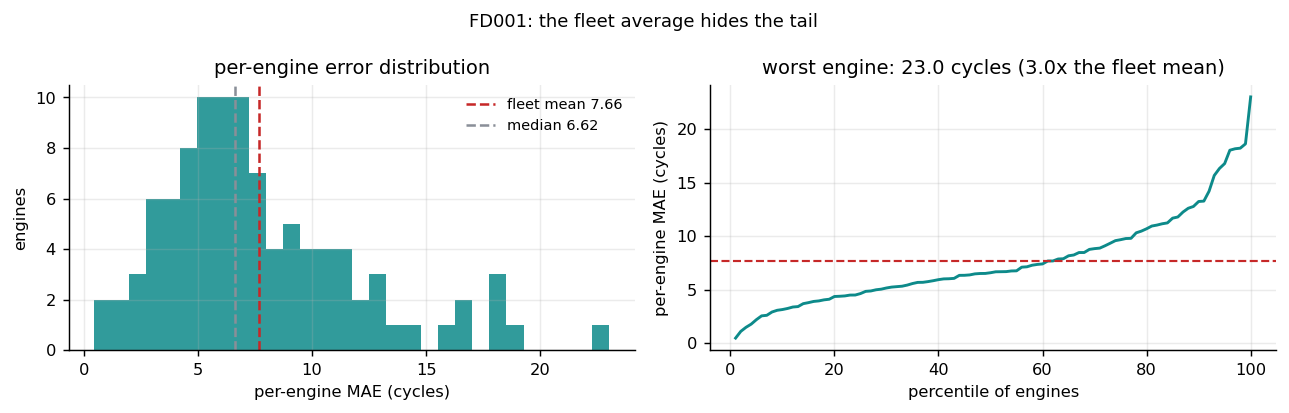
\includegraphics[width=\columnwidth]{FD001_per_engine.png}
            \caption{Per-engine MAE distribution, FD001 test engines. The fleet mean is pulled above the median by a thin tail of harder engines.}
            \label{fig:perengine}
        \end{figure}

\section{Failure-Horizon Classification}
\label{sec:classification}

    Three independent models - one per horizon - are fit and calibrated, comparing Logistic Regression (current-cycle and window views) against Hist Gradient Boosting on window features. \tabref{tab:clf_fd001} reports the selected classifier at each horizon on FD001 test engines; \texttt{logreg\_window} is selected at every horizon by validation PR-AUC.

    \begin{table}[H]
        \caption{Selected failure-horizon classifiers, FD001 test engines.}
        \label{tab:clf_fd001}
        \begin{tabular}{rrrrrr}
        \toprule
        \textbf{$h$} & \textbf{Thr.} & \textbf{PR-AUC} & \textbf{Prec.} & \textbf{Recall} & \textbf{Brier} \\
        \midrule
        10 & 0.030 & 0.695 & 0.254 & 1.000 & 0.0006 \\
        20 & 0.010 & 0.884 & 0.442 & 1.000 & 0.0024 \\
        30 & 0.015 & 0.934 & 0.667 & 0.985 & 0.0051 \\
        \bottomrule
        \end{tabular}
        \tabletext{Note: thresholds are selected on validation engines by minimising $20\cdot\mathrm{FN}+\mathrm{FP}$, not fixed at 0.5.}
    \end{table}

    PR-AUC rises with horizon length because the 10-cycle positive class is far rarer (Section 2); the practical trade-off is that longer horizons give more lead time at the cost of more ambiguous, higher-false-alarm alerts, quantified directly in Section~\ref{sec:earlywarning}. Isotonic calibration, fit on validation engines, materially improves both Brier score and expected calibration error relative to the raw classifier output for every horizon (\figref{fig:calibration}); the raw probabilities from a \texttt{class\_weight="balanced"} logistic regression are especially miscalibrated and must not be read as probabilities before this step.

    \begin{figure}[H]
        \centering
        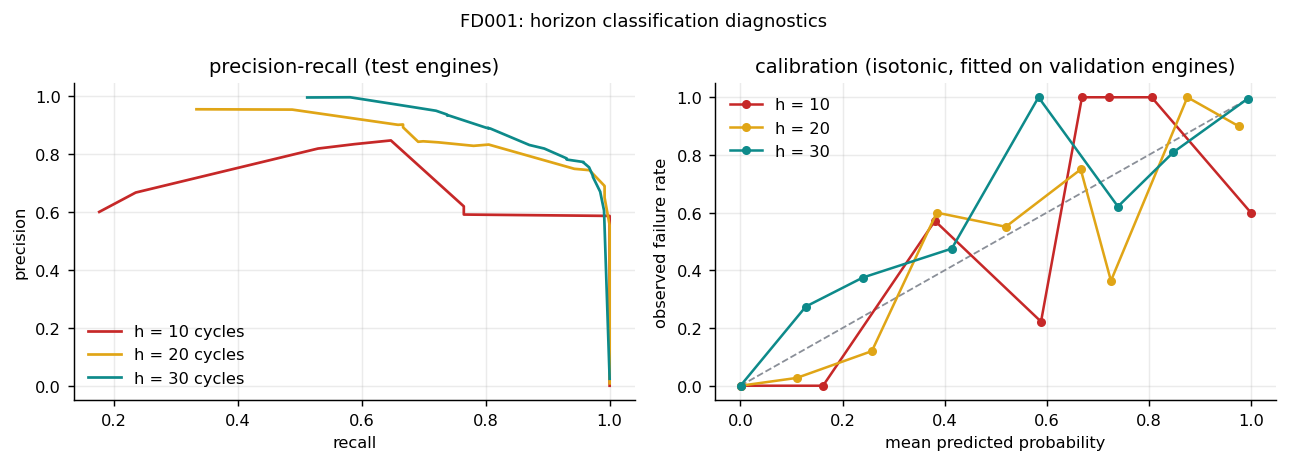
\includegraphics[width=\columnwidth]{FD001_pr_calibration.png}
        \caption{Precision-recall curves and post-calibration reliability curves for the three selected FD001 classifiers.}
        \label{fig:calibration}
    \end{figure}

    \figref{fig:confusion} shows the resulting confusion matrices at the validation-tuned thresholds. Every horizon achieves recall at or above 0.985 on the rare positive class - the row-level analogue of the zero-miss behaviour reported for the combined decision policy in Section~\ref{sec:earlywarning} - at the cost of a false-positive count that grows as the horizon shortens and the class imbalance worsens.

    \begin{figure}[H]
        \centering
        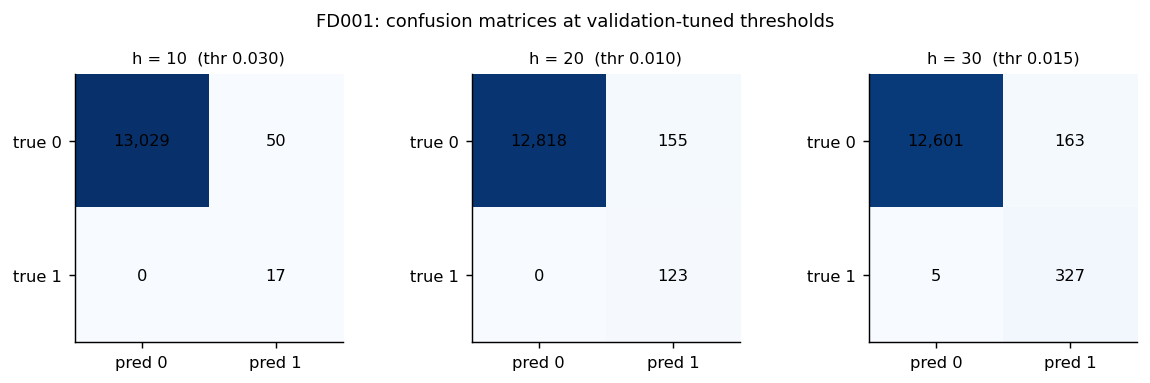
\includegraphics[width=\columnwidth]{FD001_confusion.png}
        \caption{Confusion matrices at validation-tuned thresholds, FD001 test engines, all three horizons.}
        \label{fig:confusion}
    \end{figure}

\section{Unsupervised Anomaly Detection}

    Four detectors - Isolation Forest, Local Outlier Factor, One-Class SVM, and PCA reconstruction error \cite{liu2008isolation,breunig2000lof,scholkopf2001estimating} - are fit on the healthy region of training engines only (first 30 cycles, no failure label, no test row), sharing one leakage-safe feature space (current regime residuals plus their 30-cycle rolling mean) projected through a whitened 10-component PCA for the three boundary-based methods. Every raw score is oriented so that larger means more abnormal and mapped to its \emph{validation percentile}, since raw magnitudes are not comparable across detectors.

    \begin{table}[H]
        \caption{Anomaly detector comparison, FD001 test engines.}
        \label{tab:anomaly}
        \begin{tabular}{lrrrr}
        \toprule
        \textbf{Detector} & \textbf{Sep.} & \textbf{Miss} & \textbf{Lead} & \textbf{Cost} \\
        \midrule
        Isolation Forest & 0.419 & 0.563 & 26.0 & 121.9 \\
        One-Class SVM    & 0.481 & 0.563 & 25.0 & 124.8 \\
        LOF              & 0.459 & 0.625 & 28.2 & 135.2 \\
        PCA reconstruction & 0.302 & 0.625 & 74.5 & 146.6 \\
        \bottomrule
        \end{tabular}
        \tabletext{Note: ``Sep.'' is the gap between mean normalised score near failure (RUL$\le$30) and healthy (RUL$>$100); ``Miss'' and ``Cost'' use the asymmetric policy of Section~\ref{sec:asymcost}.}
    \end{table}

    All four detectors show a positive score separation between near-failure and healthy regions (\figref{fig:anomprofile}), confirming the unsupervised score rises before failure without ever having seen a failure label. Alert thresholds are selected per detector on validation engines by the same asymmetric cost, subject to an operational false-alert-rate ceiling (5\% of healthy cycles); without this constraint the raw cost-optimal threshold alerts almost continuously, since a missed engine costs 200$\times$ a single false alert.

    \begin{figure}[H]
        \centering
        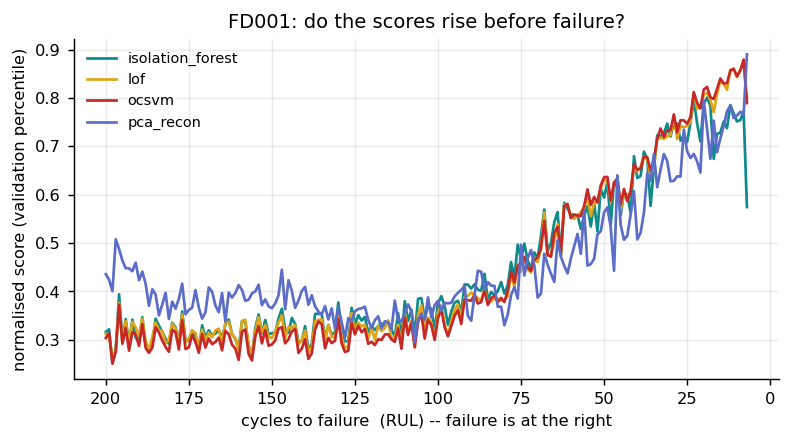
\includegraphics[width=\columnwidth]{FD001_anomaly_profiles.png}
        \caption{Normalised anomaly score aligned by cycles-to-failure, all four detectors, FD001 test engines.}
        \label{fig:anomprofile}
    \end{figure}

    The anomaly detectors' miss rates (56-63\%) are substantially higher than the supervised classifiers'. This is the expected cost of using no labels: their operational value is independence, not standalone accuracy - a persistent anomaly with low supervised risk is surfaced to the operator as a disagreement (Section~\ref{sec:policy}) rather than averaged away.

\section{Uncertainty Quantification}
\label{sec:uncertainty}

    Two interval methods are compared for RUL, both calibrated on validation engines with nominal 90\% coverage ($\alpha=0.10$). Split conformal prediction on absolute residuals gives a provable but \emph{constant-width} interval, which makes the decision policy's ``is this interval wide'' question vacuous. The deployed method is conformalized quantile regression (CQR) \cite{romano2019conformalized,vovk2005algorithmic}: two gradient-boosted quantile regressors at $\alpha/2$ and $1-\alpha/2$, conformalised on validation residuals, giving an adaptive width that tracks local trajectory difficulty while retaining the same finite-sample coverage guarantee.

    \begin{table}[H]
        \caption{RUL interval quality, FD001 test engines (held-out).}
        \label{tab:interval}
        \begin{tabular}{lrrr}
        \toprule
        \textbf{Method} & \textbf{Coverage} & \textbf{Mean w.} & \textbf{Median w.} \\
        \midrule
        Split conformal & 0.902 & 43.28 & 43.34 \\
        CQR (deployed)  & 0.933 & 36.86 & 34.77 \\
        \bottomrule
        \end{tabular}
    \end{table}

    Both methods over-cover their nominal target - expected, since engine trajectories are autocorrelated and violate the conformal exchangeability assumption, and over-coverage is the safe direction. CQR's width ranges from roughly 1-2 cycles on confidently-healthy rows to over 30 cycles in the ambiguous mid-life transition, versus a literally constant $2q=43.3$ cycles for split conformal; this adaptivity is what allows the decision policy to distinguish a genuinely uncertain prediction from a confident one. Classifier probability calibration is reported in Section~\ref{sec:classification}; anomaly-score uncertainty is the validation-percentile margin already described in Section 7, deliberately never presented as a probability.

\section{Early-Warning Analysis and Asymmetric Cost}
\label{sec:earlywarning}
\label{sec:asymcost}

    For each held-out engine, the first \emph{persistent} alert cycle $\tau(i)$ is the first cycle at which $m{=}3$ of the last $n{=}5$ cycles are flagged, giving lead time $L(i) = T(i) - \tau(i)$. Cost is
    \[
        C = c_{\text{miss}} \cdot \mathbb{1}[\text{missed}] + c_{\text{late}} \cdot \max(0, h - L) + c_{\text{early}} \cdot \max(0, L - h),
    \]
    with $c_{\text{miss}}{=}200$, $c_{\text{late}}{=}5$/cycle, $c_{\text{early}}{=}1$/cycle and target window $h{=}20$ cycles, so $c_{\text{miss}} > c_{\text{late}} > c_{\text{early}}$ as required. Test engines are only scored as ``at risk'' if their observed window actually reaches $\mathrm{RUL} \le h$ - most FD001 test engines are truncated well before that point, leaving 16 at-risk engines. \tabref{tab:earlywarn} reports lead time and cost by alert source.

    \begin{table}[H]
        \caption{Early-warning performance, FD001, 16 at-risk test engines.}
        \label{tab:earlywarn}
        \begin{tabular}{lrrrr}
        \toprule
        \textbf{Source} & \textbf{Miss} & \textbf{Lead} & \textbf{Cost} \\
        \midrule
        Classifier $h{=}20$ & 0.000 & 25.3 & 5.6 \\
        Classifier $h{=}30$ & 0.000 & 32.9 & 12.9 \\
        Policy (INSPECT/STOP) & \textbf{0.000} & 51.3 & 31.3 \\
        Policy (STOP only) & 0.313 & 19.0 & 69.3 \\
        Classifier $h{=}10$ & 0.438 & 13.3 & 106.3 \\
        Anomaly (Isolation Forest) & 0.563 & 26.0 & 121.9 \\
        \bottomrule
        \end{tabular}
        \tabletext{Note: cost is average cost (arbitrary credits) per at-risk engine, components never collapsed silently.}
    \end{table}

    The combined policy (INSPECT or STOP) is the only alert source with zero missed warnings, at the cost of the largest early-warning burden - the correct trade-off under $c_{\text{miss}} \gg c_{\text{early}}$. The narrow, specific STOP-only rule and the 10-cycle classifier alone both carry a substantial miss rate and would be unsafe as standalone warning systems. \figref{fig:leadtime} shows the resulting lead-time distribution by alert source; \figref{fig:cost} decomposes cost into its three components, so a low average can never silently hide a non-zero miss rate.

    \begin{figure}[H]
        \centering
        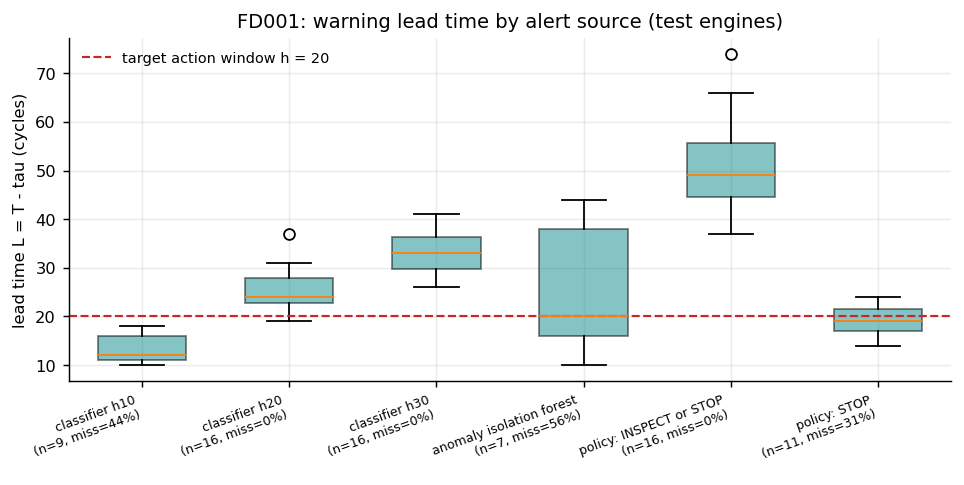
\includegraphics[width=\columnwidth]{FD001_leadtime.png}
        \caption{Lead-time distribution by alert source, FD001 at-risk test engines. The dashed line marks the target action window $h=20$.}
        \label{fig:leadtime}
    \end{figure}

    \begin{figure}[H]
        \centering
        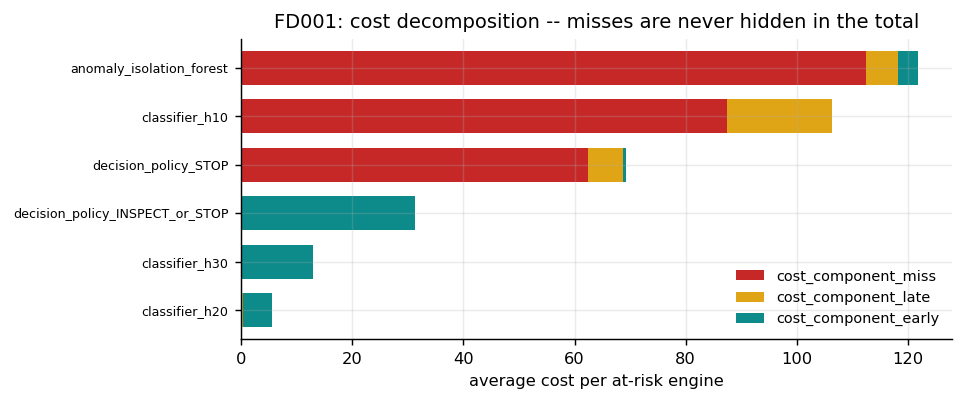
\includegraphics[width=\columnwidth]{FD001_cost.png}
        \caption{Cost decomposition by alert source, FD001. Miss, late-delay and early-burden components are shown separately.}
        \label{fig:cost}
    \end{figure}

\section{Decision Policy}
\label{sec:policy}

    The three signals are combined by a small, auditable rule set rather than a learned meta-model. STOP requires either two independent critical signals agreeing (near-term calibrated risk above threshold \emph{and} a critical lower RUL bound), or one critical signal with a \emph{non-wide} CQR interval; a critical signal paired with a wide interval is explicitly downgraded to INSPECT, because risk cannot then be separated from model uncertainty. INSPECT additionally fires on elevated 20/30-cycle risk, a moderately low lower bound, or a persistent anomaly (the same $m$-of-$n$ rule as Section~\ref{sec:earlywarning}). Every recommendation carries the specific rule that triggered it and a disagreement flag, raised when the anomaly detector is persistent while the supervised 30-cycle risk stays low - surfaced to the operator rather than silently averaged away, per the brief's explicit requirement.

    On FD001 test engines, the policy places every critical row ($\mathrm{RUL}\le10$) in STOP and no critical row in CONTINUE - the one failure mode that must not occur. At-risk rows split between INSPECT and STOP as evidence accumulates; a small fraction of healthy rows receive INSPECT or STOP, the measured price of the zero-miss behaviour in \tabref{tab:earlywarn}.

    \begin{code}
    \begin{lstlisting}[language=Python, basicstyle=\ttfamily\footnotesize, columns=fullflexible, breaklines=true]
def recommend(rul_pt, rul_lo, rul_hi, p_fail, anom_hist, policy):
    wide = (rul_hi - rul_lo) >= policy.wide_interval_cycles
    critical_bound = rul_lo <= policy.rul_lo_stop
    high_near_risk = p_fail[10] >= policy.p10_stop

    if high_near_risk and critical_bound:
        return STOP  # two independent signals: wide OK
    if (critical_bound or high_near_risk) and not wide:
        return STOP  # one signal, but interval is tight
    if (critical_bound or high_near_risk) and wide:
        return INSPECT  # risk cannot be split from uncertainty
    if elevated_20_30_risk or low_bound or persistent_anomaly:
        return INSPECT
    return CONTINUE
    \end{lstlisting}
    \caption{Simplified decision rule. The full implementation additionally records the specific trigger string and a disagreement flag for every call.}
    \label{lst:policy}
    \end{code}

\section{Stage 2 and Bonus Findings}

    \tabref{tab:master} reports the identical protocol applied to all four subsets. \figref{fig:master} visualises the same comparison.

    \begin{table*}[t]
        \centering
        \caption{Master comparison across all four subsets, identical protocol.}
        \label{tab:master}
        \begin{tabular}{lrrrrrrrrr}
        \toprule
        \textbf{Subset} & \textbf{Cond./Fault} & \textbf{Cap} & \textbf{MAE} & \textbf{Cov.} & \textbf{PR@10} & \textbf{PR@20} & \textbf{PR@30} & \textbf{Miss} & \textbf{Cost} \\
        \midrule
        FD001 & 1/1 & 130 & 8.21 & 0.933 & 0.695 & 0.884 & 0.934 & 0.000 & 31.3 \\
        FD002 & 6/1 & 110 & 5.99 & 0.918 & 0.687 & 0.881 & 0.941 & 0.000 & 38.7 \\
        FD003 & 1/2 & 125 & 5.21 & 0.933 & 0.646 & 0.901 & 0.948 & 0.000 & 32.8 \\
        FD004 & 6/2 & 125 & 6.69 & 0.913 & 0.353 & 0.739 & 0.834 & 0.000 & 31.3 \\
        \bottomrule
        \end{tabular}
        \tabletext{Note: ``Cov.'' is CQR test coverage; ``Cost'' is the combined-policy average cost per at-risk engine (Section~\ref{sec:earlywarning}); RUL caps differ by subset (Section~\ref{sec:rul}), so raw MAE is not directly comparable across rows.}
    \end{table*}

    \begin{figure}[H]
        \centering
        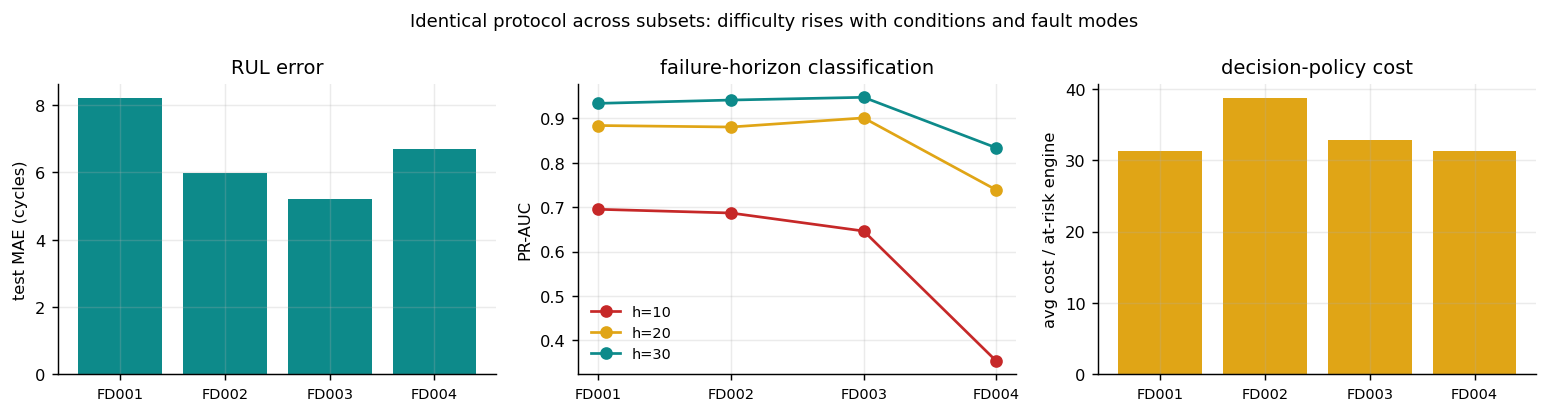
\includegraphics[width=\columnwidth]{master_comparison.png}
        \caption{Test MAE, per-horizon PR-AUC, and decision-policy cost across all four subsets under the identical protocol.}
        \label{fig:master}
    \end{figure}

    \subsection{What Breaks Under Each Stressor}

        FD003 (two fault modes, one condition) stresses the model with a mixture of two degradation mechanisms under otherwise identical conditions; the pipeline itself required no modification, and RUL/classification metrics remain close to or better than FD001. FD002 (six conditions, one fault mode) is the stressor that \emph{does} require a structural change: without regime-aware normalisation, between-regime sensor variance dominates the degradation signal. \figref{fig:regimes} confirms the discovered operating regimes align with the six documented conditions; \figref{fig:condeffect} shows one sensor's between-regime spread dwarfing its within-regime drift, the direct justification for regime-conditional residuals rather than a single global scaler.

        \begin{figure}[H]
            \centering
            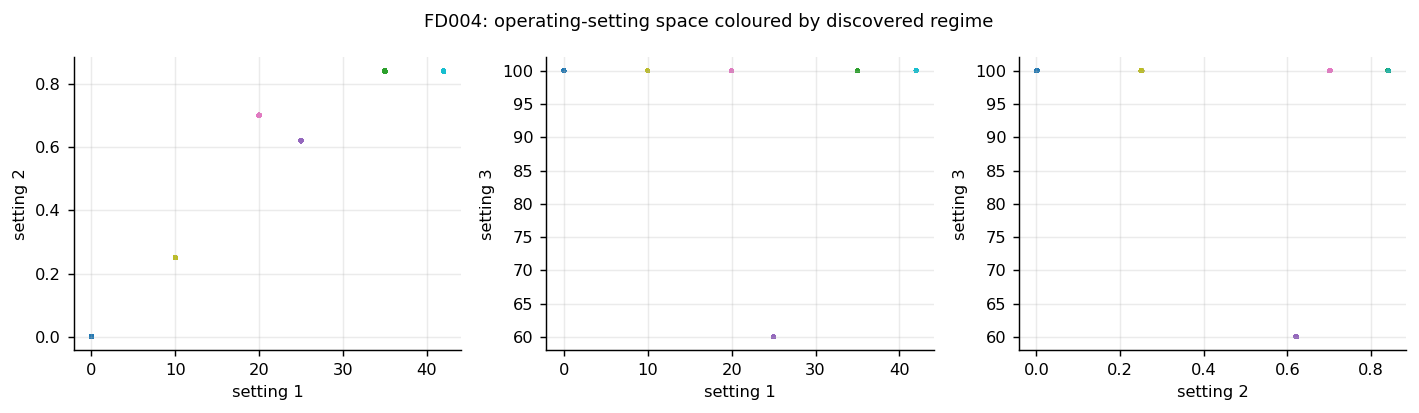
\includegraphics[width=\columnwidth]{FD004_regimes.png}
            \caption{Operating-setting space for FD004 training engines, coloured by the six k-means regimes discovered on training data alone.}
            \label{fig:regimes}
        \end{figure}

        \begin{figure}[H]
            \centering
            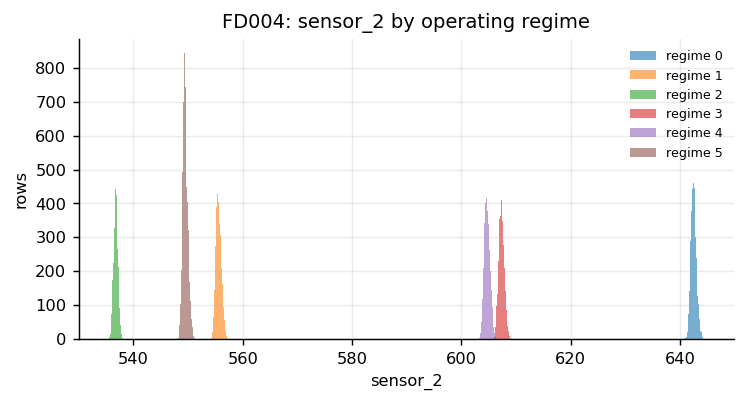
\includegraphics[width=\columnwidth]{FD004_condition_effect.png}
            \caption{Distribution of one sensor channel by discovered operating regime, FD004. Between-regime spread dominates within-regime degradation drift.}
            \label{fig:condeffect}
        \end{figure}

    \subsection{Isolating the Combined Challenge: a \texorpdfstring{$2\times2$}{2x2} Design}

        Because C-MAPSS varies exactly two independent factors, the four subsets form a complete factorial design (\{1,6\} conditions $\times$ \{1,2\} fault modes), letting the individual condition effect and fault-mode effect be separated from their combined effect. Using FD001 as baseline, the condition effect is FD002$-$FD001, the fault-mode effect is FD003$-$FD001, and their sum is the \emph{additive prediction} for FD004; the gap between that prediction and the actual FD004 result is the interaction.

        \begin{table}[H]
            \caption{Factorial interaction analysis (FD004 vs.\ additive prediction).}
            \label{tab:interaction}
            \begin{tabular}{lrrrr}
            \toprule
            \textbf{Metric} & \textbf{Cond.} & \textbf{Fault} & \textbf{Additive} & \textbf{Actual} \\
            \midrule
            PR-AUC@10 & $-0.008$ & $-0.049$ & $-0.057$ & $-0.342$ \\
            PR-AUC@20 & $-0.003$ & $+0.017$ & $+0.014$ & $-0.145$ \\
            PR-AUC@30 & $+0.008$ & $+0.014$ & $+0.021$ & $-0.100$ \\
            \bottomrule
            \end{tabular}
            \tabletext{Note: interaction = Actual $-$ Additive; e.g.\ PR-AUC@20 interaction is $-0.159$, a strong negative interaction not explained by either stressor alone.}
        \end{table}

        Individually, six conditions barely hurts 20-cycle classification ($-0.003$) and two fault modes even helps slightly ($+0.017$); combined, PR-AUC@20 falls by $0.145$ - roughly ten times the additive prediction. The mechanism is visible in the pipeline itself: regime-aware normalisation estimates per-regime sensor statistics, but on FD004 those statistics must be estimated from a mixture of two fault modes within each regime, so the ``healthy'' reference for every regime is itself blurred by fault heterogeneity. Neither FD002 (one fault per regime) nor FD003 (one regime, two faults) exposes this interference, which is why FD004 - not a larger model on the same data - is the correct bonus benchmark. RUL MAE is not used for this interaction analysis because the RUL cap differs by subset (Section~\ref{sec:rul}), confounding raw-MAE comparability; PR-AUC and the decision-policy metrics are cap-independent.

    \subsection{Per-Regime Performance and Threshold Stability}

        \tabref{tab:regime} breaks FD004 test performance down by discovered regime. Error is broadly comparable across regimes (MAE range 6.55-6.79), supporting one shared model over six dedicated ones, but PR-AUC@10 varies from 0.19 to 0.76 - regime 4 is measurably easier at the shortest horizon than regime 0.

        \begin{table}[H]
            \caption{FD004 test performance by operating regime.}
            \label{tab:regime}
            \begin{tabular}{rrrrr}
            \toprule
            \textbf{Regime} & \textbf{Rows} & \textbf{MAE} & \textbf{PR@10} & \textbf{PR@20} \\
            \midrule
            0 & 6{,}054  & 6.79 & 0.186 & 0.684 \\
            1 & 6{,}232  & 6.67 & 0.549 & 0.739 \\
            2 & 6{,}107  & 6.79 & 0.204 & 0.790 \\
            3 & 6{,}254  & 6.55 & 0.450 & 0.782 \\
            4 & 6{,}185  & 6.69 & 0.760 & 0.816 \\
            5 & 10{,}382 & 6.67 & 0.369 & 0.711 \\
            \bottomrule
            \end{tabular}
        \end{table}

        Comparing a single global anomaly threshold against per-regime thresholds (both derived from validation engines) shows the alert rate spread across regimes under the global threshold is small (0.0027, i.e.\ 1.2-1.5\% alert rate across regimes) but not zero; the deployed thresholds remain global on the grounds that six regime-specific estimates, each fit on a fraction of the validation data, trade a measured, bounded bias for an unmeasured increase in estimator variance.

    \subsection{Transfer vs.\ a Dedicated Model}

        \tabref{tab:transfer} applies each subset's fully-fitted, locked system - its own sensor list, regime clusters, RUL cap, calibrators and thresholds - to FD004 test engines with zero refitting.

        \begin{table}[H]
            \caption{Zero-shot transfer to FD004 test engines.}
            \label{tab:transfer}
            \begin{tabular}{lrrr}
            \toprule
            \textbf{Source} & \textbf{MAE} & \textbf{PR@20} & \textbf{Dedicated} \\
            \midrule
            FD004 & \textbf{6.69} & \textbf{0.739} & yes \\
            FD002 & 7.48 & 0.225 & no \\
            FD003 & 34.32 & 0.009 & no \\
            FD001 & 42.35 & 0.009 & no \\
            \bottomrule
            \end{tabular}
        \end{table}

        The dedicated FD004 model wins, as expected, but the transfer \emph{ordering} is the informative result: FD002 (six conditions, wrong fault-mode count) transfers dramatically better than FD001 or FD003 (one condition, wrong or partial fault coverage), despite FD002 never having seen a fan-degradation fault. Operating-context coverage transfers better than fault-mode coverage - a source pipeline fitted under one condition has regime statistics for that condition alone, so five of FD004's six regimes are normalised with statistics that never described them, which is a larger error source than an unseen fault mechanism. Practically: when facing an uncharacterised fleet, prioritise collecting operating-condition diversity over fault diversity.

    \subsection{Ablations}

        \tabref{tab:ablation} reports FD001 and FD004 ablations under the identical protocol; each removes one design element while holding everything else fixed.

        \begin{table}[H]
            \caption{Ablations (test MAE and PR-AUC@20 deltas vs.\ full model).}
            \label{tab:ablation}
            \begin{tabular}{
                >{\raggedright\arraybackslash}p{0.30\columnwidth}
                >{\raggedright\arraybackslash}p{0.08\columnwidth}
                rr
            }
            \toprule
            \textbf{Ablation} & \textbf{Set} & $\Delta$\textbf{MAE} & $\Delta$\textbf{PR@20} \\
            \midrule
            No operating settings   & FD001 & $+0.01$ & $-0.003$ \\
            No trend features       & FD001 & $+2.48$ & $-0.006$ \\
            Short window (10 cyc.)  & FD001 & $-0.48$ & $+0.022$ \\
            No operating settings   & FD004 & $-0.03$ & $-0.007$ \\
            No trend features       & FD004 & $+2.57$ & $-0.058$ \\
            Short window (10 cyc.)  & FD004 & $-0.25$ & $-0.024$ \\
            Global scaling (no regime norm.) & FD004 & $+3.05$ & $-0.042$ \\
            \bottomrule
            \end{tabular}
        \end{table}

        Removing the trend feature block (slope, EWM, first difference, drift) is the single most damaging ablation on both subsets, confirming that degradation is read from a trend rather than an instantaneous level. Removing the three operating settings is harmless on FD001 (single condition, no information beyond noise) but measurably harmful on FD004 - the controlled contrast the two subsets provide. On FD004 specifically, replacing regime-aware normalisation with one global scaler is the second most damaging ablation and inflates the decision-policy cost nearly three-fold (from 31.3 to 90.2), the clearest single piece of evidence that condition-aware normalisation, not model capacity, is what makes the combined challenge tractable.

\section{Error Analysis and Limitations}

    Three limitations are stated explicitly rather than absorbed into aggregate numbers. First, only a minority of test engines are ever observed inside the 20-cycle action window (16 of 100 on FD001), so early-warning miss rates rest on small denominators; a companion analysis on validation engines (which are run-to-failure and therefore fully observable) is reported in the notebook as an optimistic bracket around the locked test numbers. Second, the conformal exchangeability assumption is formally violated by within-engine autocorrelation; empirical coverage is measured on held-out engines rather than trusted from theory, and it over-covers, the safe direction. Third, fault mode is never observed in FD003/FD004, so "robust to two fault modes" is demonstrated only in aggregate, not per-mechanism - a labelled fault-mode indicator, if it existed, would allow a much sharper version of the per-regime analysis in Section~9.3.

\section{Dashboard and Application Parity}
\label{sec:app}

    A Streamlit dashboard loads only the exported artefacts (fitted preprocessing, models, calibrators, the CQR regressor, anomaly bank, and decision policy) and contains no training code, satisfying the deployment requirement that the app and the notebook remain provably consistent. \tabref{tab:dashboard} lists the evidence surfaced for each selected engine and cycle.

    \begin{table}[H]
        \caption{Dashboard elements and their evidence source.}
        \label{tab:dashboard}
        \begin{tabular}{
            >{\raggedright\arraybackslash}p{0.20\columnwidth}
            >{\raggedright\arraybackslash}p{0.42\columnwidth}
        }
        \toprule
        \textbf{Element} & \textbf{Content} \\
        \midrule
        Engine timeline & sensor/health features, current cycle highlighted \\
        RUL card & point estimate, 90\% CQR interval, cycles \\
        Failure risk & calibrated $P(\mathrm{fail}\le h)$ for $h{=}10,20,30$ with thresholds \\
        Anomaly card & normalised score, validation percentile, persistence \\
        Action & CONTINUE / INSPECT / STOP, trigger, confidence \\
        Model metadata & dataset, model version, feature window, train date \\
        \bottomrule
        \end{tabular}
    \end{table}

    An automated parity check recomputes every engine's full inference chain independently inside the app and compares it row-by-row against the notebook's precomputed timeline, asserting numerical agreement to $10^{-9}$ and 100\% agreement on the CONTINUE/INSPECT/STOP recommendation across a sample of held-out engines; both assertions pass on every subset.

\section{Conclusion}

    A single leakage-safe pipeline - one engine-level split, one causal feature space, one uncertainty method, one cost policy - produces a defensible early-warning system on FD001 and generalises, with one architectural change (regime-aware normalisation), to condition-shifted and multi-fault subsets. The FD004 bonus result is the central finding of this study: combining condition shift and multi-fault degradation is not additive, and the interaction is traceable to a specific mechanism - regime statistics blurred by fault heterogeneity - rather than asserted from a lower aggregate score.

%----------------------------------------------------------

\printbibliography

%----------------------------------------------------------

\end{document}
